%!TEX root = ../dissertation.tex
%\begin{savequote}[75mm]
%Nulla facilisi. In vel sem. Morbi id urna in diam dignissim feugiat. Proin molestie tortor eu velit. Aliquam erat volutpat. Nullam ultrices, diam tempus vulputate egestas, eros pede varius leo.
%\qauthor{Quoteauthor Lastname}
%\end{savequote}

\chapter{Experiments}

Summarizing the work done until now, it has been created a sentiment analysis dataset based on italian automotive forums by crawling web resources and then scraping HTML pages. Then, the dataset has been labeled by many workers, obtaining a sufficiently large amount of data to be processed. The next phase consisted in defining some machine learning models in order to make both topic detection and sentiment classification. In this Chapter, will be firstly presented, as a benchmark, results obtained running the models on a Twitter's dataset, and then the results obtained on the created dataset.\\
Every test will be presented with a common framework: 
\begin{itemize}
	\item Results obtained with a classification before features selection;
	\item Features selection and most important features;
	\item Results obtained after features selection;
\end{itemize}
Classification results will be presented both visually using confusion matrices and using numerical scores.\\
Since used algorithms don't require huge amount of computational power, runs have been made on a 2019 consumer technology with the following specifics:
% CPU, RAM,
\begin{center}
	\begin{tabular}{ |c||c| } 
		\hline
		\textbf{CPU} & Intel(R) Core(TM) i7-8550U CPU @ 1.80GHz 4 cores, 8 threads\\ 
		\hline
		\textbf{RAM} & 16GB DDR4 \\
		\hline
		\textbf{O.S.} & Ubuntu 18.04 \\
		\hline
	\end{tabular}
\end{center}
Where it has been installed a Python 3.7 release on a Jupyter Notebook.


\section{Experiments on Twitter's Airline Dataset}

The first series of experiments concerns the Twitter's Airline dataset described in Section 2.1.6. The purpose of these tests is to verify the goodness of the models in a dataset that is plenty of well labeled comments. The reference result on tweets sentiment classification can be extracted from \cite{Zimbra:2018:STS:3210372.3185045}, where BPEF algorithm reached the best results with an average accuracy of 71.38\% on sentiment classification on five different datasets, but average performance of all models stay around 65\%, so a similar result will be positive.\\
The dataset consists in 14640 labeled tweets, divided into 3099 positives, 2363 neutrals and 9178 negatives. Due to the plenty of data, all classes were balanced, with the number of comments of the minority class. Successively, the dataset were divided into training set and test set, respectively the 80\% and the 20\%. Moreover, the training set were further divided into actual training set and validation set, again respectively the 80\% and the 20\%. The distribution of the datasets is:

\begin{center}
	\begin{tabular}{ | c  c  c  c | c | } 
		\hline
		& \textbf{Positives} & \textbf{Nautrals} & \textbf{Negatives} & \textbf{Total} \\
		\hline
		\textbf{Training} & 960 & 960 & 960 & 2880 \\ 
		\hline
		\textbf{Validation} & 240 & 240 & 240 & 720 \\ 
		\hline
		\textbf{Test} & 300 & 300 & 300 & 900 \\
		\hline
		%\label{table:twitt-class-data}
		%\caption{Class distribution of training, validation and test sets of tweets' sentiment classification.}
	\end{tabular}
\end{center}

Due to the class balance, also accuracy score is meaningful, so it is presented along with F1-macro and F1-micro scores.


\subsection{Sentiment Classification with SVM}

After preprocessing and vectorization with TF-IDF method on the training set, involving both unigrams and bigrams, the outcome dimension counts 22.486 features. Data are stored in a sparse matrix 2880x22.486 with 50.006 stored elements, so as expected, it is actually very sparse.\\
A first model train is performed involving all features, optimizing the regularization parameter $C$ from 7 candidates exponentially equally spaced from $10^{-3}$ to $10^3$, searching for the best F1-macro score.\\
The selected model is the one with $C$=1, and the classification results obtained with the validation set are:

% SVM no fs
\begin{figure}[ht]
	\centering
	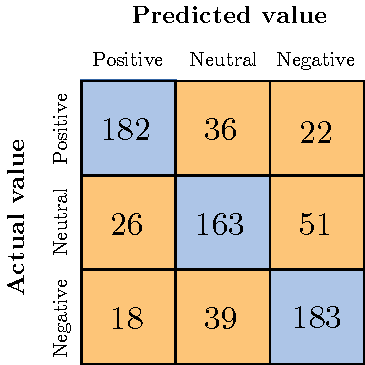
\includegraphics[scale=1]{figures/conf_matrices/twitter_snt_svm/twitter_snt_svm_bfs.pdf}
	\label{fig:tw_snt_svm_bfs}
\end{figure}

\begin{center}
	\begin{tabular}{ | c | c | } 
		\hline
		\textbf{F1-macro} & 0.734 \\
		\hline
		\textbf{F1-micro} & 0.733 \\ 
		\hline
		\textbf{Accuracy} & 0.734 \\ 
		\hline
	\end{tabular}
\end{center}

It is possible to see that the baseline method without feature selection reaches good results, aligned with state of the art. From the confusion matrix, diagonal values (which are the correctly classified) are in fact the majority, and also the accuracy of 70,4\% reflects the visual considerations.\\
The sorted weights of the three binary classifiers that constitute the one-versus-one multiclass classifier are shown in Figure \ref{fig:svm-fs}.

% fs

\begin{figure}[H]
	\centering
	\begin{subfigure}{1\textwidth} % width of left subfigure
		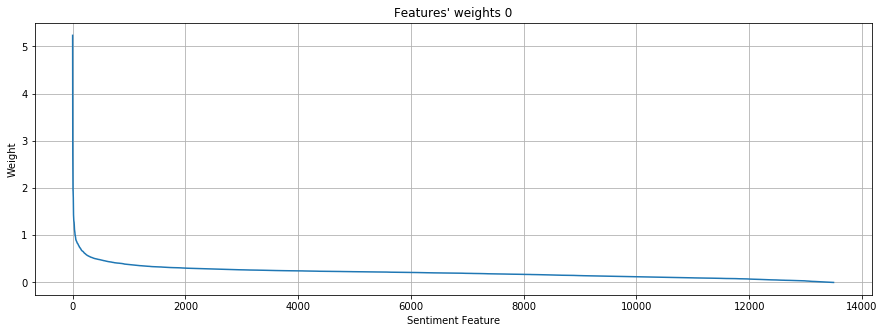
\includegraphics[width=\textwidth]{figures/conf_matrices/twitter_snt_svm/svm_fs_1.png}
	\end{subfigure}
	\begin{subfigure}{1\textwidth} % width of right subfigure
		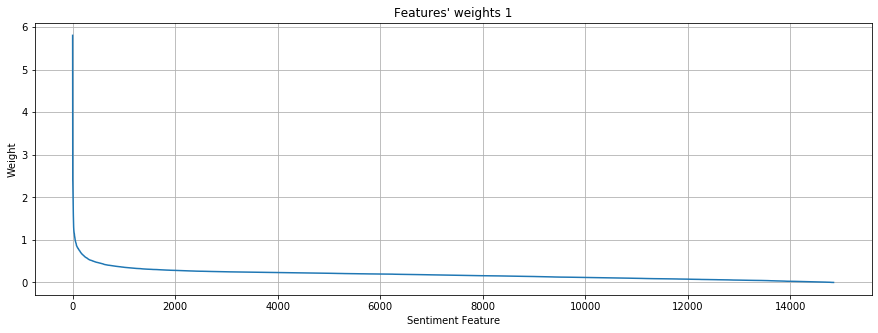
\includegraphics[width=\textwidth]{figures/conf_matrices/twitter_snt_svm/svm_fs_2.png}
	\end{subfigure}
	\begin{subfigure}{1\textwidth} % width of right subfigure
		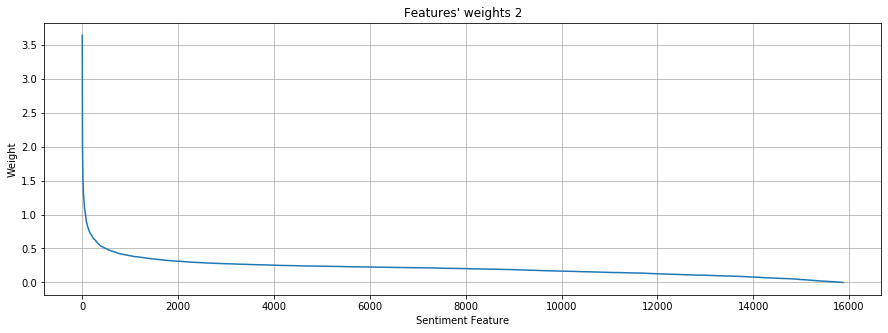
\includegraphics[width=\textwidth]{figures/conf_matrices/twitter_snt_svm/svm_fs_3.png}
	\end{subfigure}
	\caption{Features' weights of the three binary classifiers of the one-versus-one multiclass classifier} % caption for whole figure
	\label{fig:svm-fs}
\end{figure}

% SVM fs

After some manual tries, the selected cutoff values are respectively 0.3, 0.3 and 0.2, obtaining 9564 final selected features. Retraining the model using just selected features, the results on the validation set are:%, where most important with respect every binary classifier are shown in Figure % TODO features piu importanti svm
%\textcolor{red}{FEATURE PIU IMPORTANTI}


\begin{figure}[H]
	\centering
	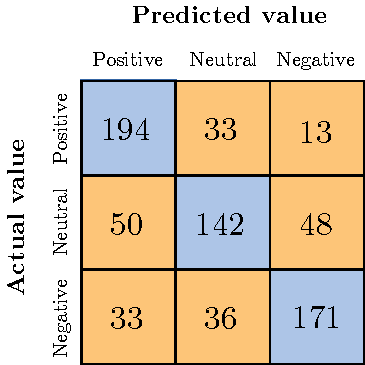
\includegraphics[scale=1]{figures/conf_matrices/twitter_snt_svm/twitter_snt_svm_afs.pdf}
	\label{fig:tw_snt_svm_afs}
\end{figure}

\begin{center}
	\begin{tabular}{ | c | c | } 
		\hline
		\textbf{F1-macro} & 0.702 \\
		\hline
		\textbf{F1-micro} & 0.704 \\ 
		\hline
		\textbf{Accuracy} & 0.704 \\ 
		\hline
	\end{tabular}
\end{center}

After feature selection it is possible to notice a loss of performance due to the removal of some relevant features. However, features selection has the goal to make the model more stable, rather that more performing. The final metrics still highlight performance close to state of the art models.


\subsection{Sentiment Classification with Revised BPEF}

At this point the goal is to enhance the previous model with the revised BPEF ensemble. In this model, feature's relevance is calculated using the information gain metric, and since it is based on dataset's distribution instead of model's weights, it is possible to calculate it as the first phase, for every combination of the model's features parameters.\\
The outcome of features ranking is very similar for all features parameters and has the trend shown in Figure \ref{fig:twitter_bpef_fs_1}.

\begin{figure}[H]
	\centering
	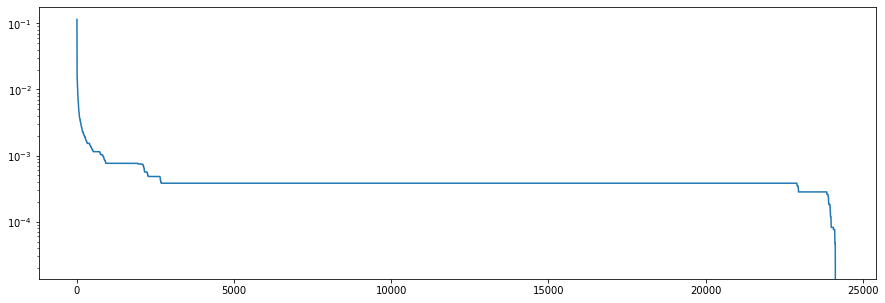
\includegraphics[width=\textwidth]{figures/conf_matrices/twitter_snt_bpef/bpef_fs_1.png}
	\caption{Information Gain trend of the features.}
	\label{fig:twitter_bpef_fs_1}
\end{figure}

It is possible to notice that there are just few features with higher information gain, while most have a flat trend. The strategy for features selection was to set the cutoff value in correspondence of the starting of the flat curve, in order to keep just features with higher information gain.\\
Before features selection it were counted the following number of features:

\begin{center}
	\begin{tabular}{ c  c  c } 
		\hline
		\textbf{Feature name} & \textbf{Word summarizing} & \textbf{\# Features} \\
		\hline
		word & false & 24.206 \\ 
		\hline
		word & true & 22.485 \\ 
		\hline
		pos & false & 30.282 \\ 
		\hline
		pos & true & 28.318 \\ 
		\hline
		swnt & false & 22.789 \\ 
		\hline
		swnt & true & 21.113 \\ 
		\hline
	\end{tabular}
\end{center}

Recalling that the involved algorithms are SVM, Logistic Regression, Ra{\"i}ve Bayes and Random Forest, they are all trained optimizing with a grid search on the followings parameters:
\begin{itemize}
	\item SVM: $C$ from $10^{-3}$ to $10^3$ with 7 exponentially evenly spaced values;
	\item Logistic Regression: $C$ from $10^{-3}$ to $10^3$ with 7 exponentially evenly spaced values;
	\item Random Forest: 
	\begin{itemize}
		\item Number of estimators: [201, 501]
		\item Maximum of looked features on split: [auto, $log_2$]
		\item Maximum depth of the tree: [10, 100]
		\item Split criterion: [gini, entropy]
	\end{itemize}
\end{itemize}

% BPEF no fs
The classification without features selection on validation data gives the following results:

\begin{figure}[H]
	\centering
	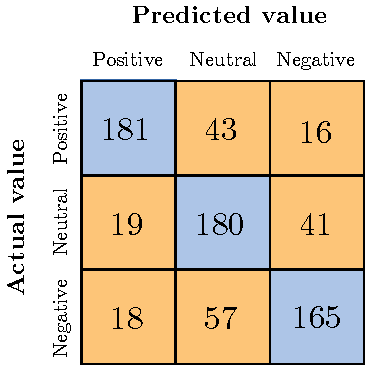
\includegraphics[scale=1]{figures/conf_matrices/twitter_snt_bpef/twitter_snt_bpef_bfs.pdf}
	\label{fig:tw_snt_bpef_bfs}
\end{figure}

\begin{center}
	\begin{tabular}{ | c | c | } 
		\hline
		\textbf{F1-macro} & 0.732 \\
		\hline
		\textbf{F1-micro} & 0.731 \\ 
		\hline
		\textbf{Accuracy} & 0.731 \\ 
		\hline
	\end{tabular}
\end{center}

% fs

The results are very similar to the ones reached with SVM classificator without features selection. Setting a cutoff value for feature selection equal to $4\times10^{-4}$, the number of selected features becomes:

\begin{center}
	\begin{tabular}{ c  c  c } 
		\hline
		\textbf{Feature name} & \textbf{Word summarizing} & \textbf{\# Features} \\
		\hline
		word & false & 2.665 \\ 
		\hline
		word & true & 2.622 \\ 
		\hline
		pos & false & 3.181 \\ 
		\hline
		pos & true & 3.057 \\ 
		\hline
		swnt & false & 2.657 \\ 
		\hline
		swnt & true & 2.612 \\ 
		\hline
	\end{tabular}
\end{center}

% BPEF fs

Which are less than one third than the previously case. Training again the model optimizing the same hyperparameters with the same grid search, the obtained results are the followings:

\begin{figure}[H]
	\centering
	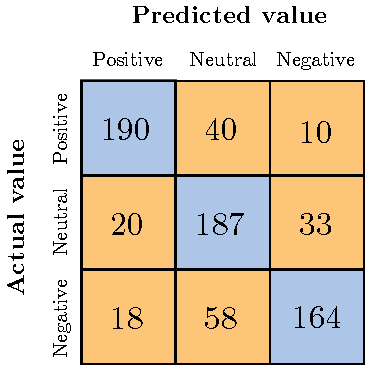
\includegraphics[scale=1]{figures/conf_matrices/twitter_snt_bpef/twitter_snt_bpef_afs.pdf}
	\label{fig:tw_snt_bpef_afs}
\end{figure}

\begin{center}
	\begin{tabular}{ | c | c | } 
		\hline
		\textbf{F1-macro} & 0.753 \\
		\hline
		\textbf{F1-micro} & 0.751 \\ 
		\hline
		\textbf{Accuracy} & 0.751 \\ 
		\hline
	\end{tabular}
\end{center}

Looking at the scores, it is easy to notice the better performance of the BPEF revisitation against the SVM model, even considering very less features. Moreover, due to the strong cut of the features and the optimal results, it is possible to suppose that the feature selection method returns an actual set of relevant features, that combined with the stability of the ensemble lead to prefer this model against the previous one.


% TODO fai test

\subsection{Sentiment Classification with Test Data}

\subsubsection{SVM Classifier}

\begin{figure}[H]
	\centering
	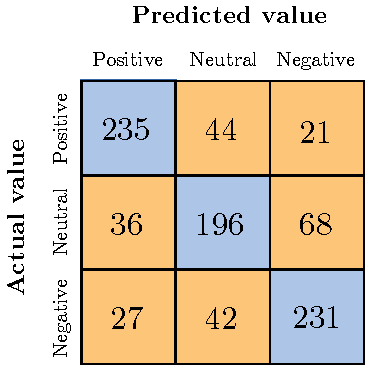
\includegraphics[scale=1]{figures/conf_matrices/twitter_snt_svm/twitter_snt_svm_tst.pdf}
	\label{fig:tw_snt_svm_tst}
\end{figure}

\begin{center}
	\begin{tabular}{ | c | c | } 
		\hline
		\textbf{F1-macro} & 0.735 \\
		\hline
		\textbf{F1-micro} & 0.736 \\ 
		\hline
		\textbf{Accuracy} & 0.736 \\ 
		\hline
	\end{tabular}
\end{center}

\subsubsection{Revised BPEF Classifier}

\begin{figure}[H]
	\centering
	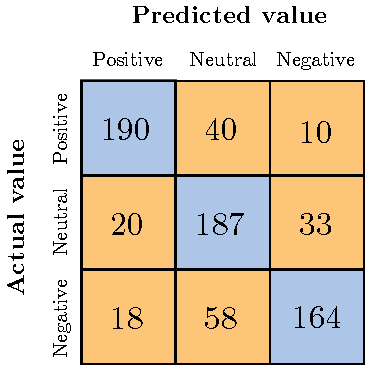
\includegraphics[scale=1]{figures/conf_matrices/twitter_snt_bpef/twitter_snt_bpef_afs.pdf}
	\label{fig:tw_snt_bpef_tst}
\end{figure}

\begin{center}
	\begin{tabular}{ | c | c | } 
		\hline
		\textbf{F1-macro} & 0.734 \\
		\hline
		\textbf{F1-micro} & 0.732 \\ 
		\hline
		\textbf{Accuracy} & 0.732 \\ 
		\hline
	\end{tabular}
\end{center}







\section{Experiments on Italian's Automotive Dataset}

Now that some results are available, it is possible to state the effectiveness of the implemented algorithms. In this section the same models for sentiment analysis will be executed on the Italian automotive dataset. Moreover, have been designed models for relevance detection that will be implemented for the cascade classifier. For all classification have been involved "Text" and "Quote" columns of the dataset, in the way that was mentioned in the previous chapter: both techniques for texts combinations were tested, and similar but better results were obtained without adding the suffix that subdivides text's words against quote's words. \\

\subsubsection{Relevance Detection}

Before sentiment classification, it has been studied the task of relevance detection, where the goal consists on identifying weather a comment talks about a given topic. In the dataset, relevance is identified in the presence of a sentiment expression, whether it is "positive", "negative" or "neutral", while the irrelevance is obviously identified in the "irrelevant" label. The problem is then summarized in a binary text classification problem, that will constitute the first block of the cascade classifier.\\
Relevance is studied one topic at time, in fact the whole study of the models was made on the class "Engine", and then exported for all others. For the class "Engine" the dataset is constituted of 7183 comments, 866 of which are classified as "relevant", so as said, unbalance is really visible. The dataset is splitted into training data and test data, respectively the 80\% and 20\%. Then, the training dataset has been further splitted into actual training and validation sets, respectively the 80\% and 20\%. The distribution of the datasets is:

\begin{center}
	\begin{tabular}{ | c  c  c | c | } 
		\hline
		& \textbf{Relevant} & \textbf{Irrelevant} & \textbf{Total} \\
		\hline
		\textbf{Training} & 532 & 4.064 & 4.596 \\ 
		\hline
		\textbf{Validation} & 133 & 1.017 & 1.150 \\ 
		\hline
		\textbf{Test} & 166 & 1.271 & 1.437\\
		\hline
		%\label{table:twitt-class-data}
		%\caption{Class distribution of training, validation and test sets of tweets' sentiment classification.}
	\end{tabular}
\end{center}

Training of the models has been made again optimizing the hyperparameters with a grid search, maximizing the F1-macro score, which is more informative for this imbalance case, in fact small changes on minority class classification give appreciable differences on the macro score, while considering the micro score, the final output is predominated by the values of the majority class. However, for comparison, if two models obtain similar F1-macro scores, the better choice falls on the one which gives the best recall, which means that it catches better the topic relevance, even returning more false positives.



\subsubsection{Sentiment Classification}

Sentiment classification involves the same techniques used for the same task with the Twitter's Airline dataset presented in the preceding section. Even for sentiment classification the algorithms were tested on the "Engine" class, but just considering the relevant comments. For this reason the dataset became similar to an usual sentiment analysis's dataset. It contains 830 total comments, divided into 317 positives, 358 neutrals and 155 negatives. Also for this phase, the dataset has been divided into training set and test set, respectively the 80\% and 20\%, and training set has been splitted into actual training set and validation set, again respectively the 80\% and 20\%. The distribution of the datasets is:

\begin{center}
	\begin{tabular}{ | c  c  c c | c | } 
		\hline
		& \textbf{Positives} & \textbf{Neutrals} & \textbf{Negatives} & \textbf{Total} \\
		\hline
		\textbf{Training} & 204 & 228 & 100 & 532 \\ 
		\hline
		\textbf{Validation} & 51 & 57 & 25 & 133 \\ 
		\hline
		\textbf{Test} & 62 & 73 & 30 & 165 \\
		\hline
		%\label{table:twitt-class-data}
		%\caption{Class distribution of training, validation and test sets of tweets' sentiment classification.}
	\end{tabular}
\end{center}

Since classes are largely unbalanced, undersampling the dataset for train the classifier on balanced data may lead to underfitting, so the difficulty is to control the bias due to the presence of the large "irrelevant" class.



\subsection{Relevance Detection with SVM}

% SVM no fs
The whole dataset is preprocessed involving words summarizing and vectorization with TF-IDF method for unigrams and bigrams. The outcome's dimension count 156.369 features. The number of features is a lot larger than the one seen for twitter's dataset, even in obtained with the same method. This is a consequence of the scarcity of words and expressions on Twitter's comments, and the opposite on Forums, where texts usually are more articulated. Since the number of features is very large, and the data are just few hundreds, the features selection technique may be essential for improve the stability picking just the features that are actually useful for the classification. All trainings have been made optimizing the parameter $C$ with a grid search on the values from $10^{-3}$ to $10^3$ with 7 exponentially evenly spaced values. A first training considering all features gives the following results:

\begin{figure}[H]
	\centering
	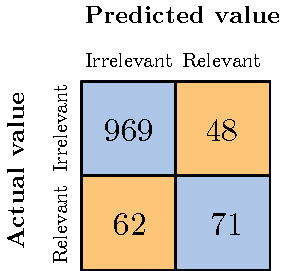
\includegraphics[scale=1]{figures/conf_matrices/ita_rel_svm/ita_rel_svm_bfs.pdf}
	\label{fig:ita_rel_svm_bfs}
\end{figure}

\begin{center}
	\begin{tabular}{ | c | c | } 
		\hline
		\textbf{F1-macro} & 0.563 \\
		\hline
		\textbf{Recall} & 0.534 \\ 
		\hline
		\textbf{Precision} & 0.597 \\ 
		\hline
	\end{tabular}
\end{center}

% fs
The best classifier, obtained with $C$=1000, gives the weights shown in Figure \ref{fig:ita_rel_svm_fs}, that follow the usual trend.

\begin{figure}[H]
	\centering
	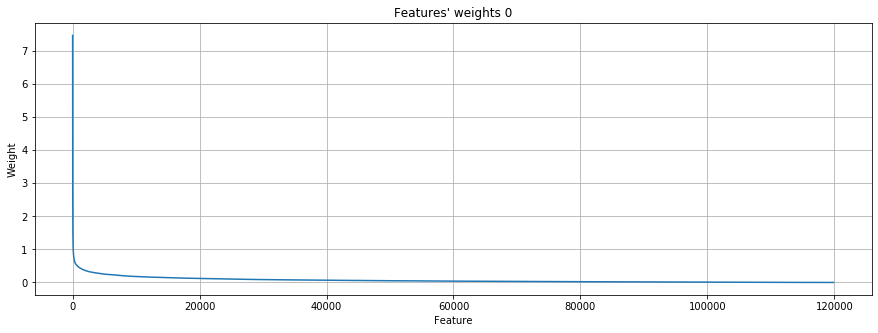
\includegraphics[width=\textwidth]{figures/conf_matrices/ita_rel_svm/ita_rel_svm_fs.png}
	\caption{Features' weights of SVM classifier for relevance detection before features selection}
	\label{fig:ita_rel_svm_fs}
\end{figure}

The cutoff value for features selection has been set to 0.2, reducing the final features' dimension to 8234. Training again the classifier on selected features, it reaches the following results:

% SVM fs

\begin{figure}[H]
	\centering
	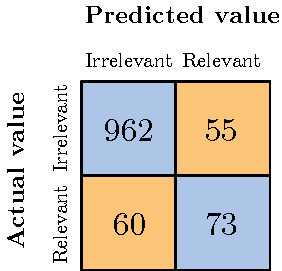
\includegraphics[scale=1]{figures/conf_matrices/ita_rel_svm/ita_rel_svm_afs.pdf}
	\label{fig:ita_rel_svm_afs}
\end{figure}

\begin{center}
	\begin{tabular}{ | c | c | } 
		\hline
		\textbf{F1-macro} & 0.559 \\
		\hline
		\textbf{Recall} & 0.549 \\ 
		\hline
		\textbf{Precision} & 0.570 \\ 
		\hline
	\end{tabular}
\end{center}

The most relevant features, obtained by the 25 heaviest weights of the SVM classifier, are shown in Figure \ref{fig:ita_rel_svm_feat}, where it is interesting to notice some actual reference about engines, especially for red values that have the weight concordant to the relevance.

\begin{figure}[H]
	\centering
	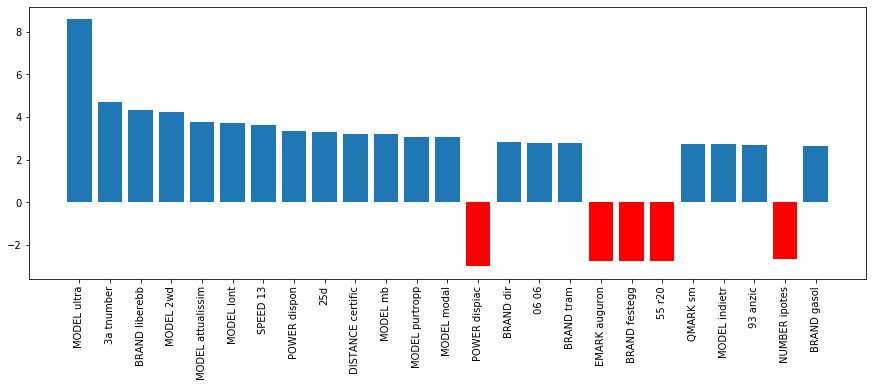
\includegraphics[width=\textwidth]{figures/conf_matrices/ita_rel_svm/svm_rel_best_feat.png}
	\caption{25 most relevant features of SVM relevance classifier after features selection}
	\label{fig:ita_rel_svm_feat}
\end{figure}

The final model was the one with the parameter $C$=100. Just few considerations about the previous results: Even if the task is different from the Twitter sentiment analysis, the many more difficulties are reflected in the final results, in fact performances are significantly lower. After features selection the F1-macro score obtained slightly poorer results, but the recall's improvement and the supposed improved stability makes the second model a bit better.\\
In the following paragraph, the SVM relevance detection classifier will be compared to a Logistic Regression model with the same final purpose.


\subsection{Relevance Detection with Logistic Regression}

The same process for relevance detection seen in the previous paragraph, has been applied involving the Logistic Regression classifier. The procedure was the same: a first na{\"i}ve classification for empirically find the most important features, then the cutoff of the less relevant ones, followed by the final training that defines the actual model. also the grid for hyperparameter's optimization was the same of the previous case.\\
Without features selection, the classifier with optimal $C$=100, obtained the following scores:

% LR no fs
\begin{figure}[H]
	\centering
	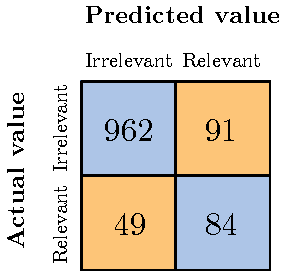
\includegraphics[scale=1]{figures/conf_matrices/ita_rel_logreg/ita_rel_logreg_bfs.pdf}
	\label{fig:ita_rel_logreg_bfs}
\end{figure}

\begin{center}
	\begin{tabular}{ | c | c | } 
		\hline
		\textbf{F1-macro} & 0.545 \\
		\hline
		\textbf{Recall} & 0.631 \\ 
		\hline
		\textbf{Precision} & 0.480 \\ 
		\hline
	\end{tabular}
\end{center}

Features' selection has been made exploiting L1-regularization on model training. The effect is shown in Figure \ref{fig:ita_rel_logreg_fs}, where it is possible to verify the early discussed characteristic: L1-regularization selects almost automatically most important features nullifying less important ones. Setting the cutoff value to 0.1, the method returns 1349 final values.\\

% fs
\begin{figure}[H]
	\centering
	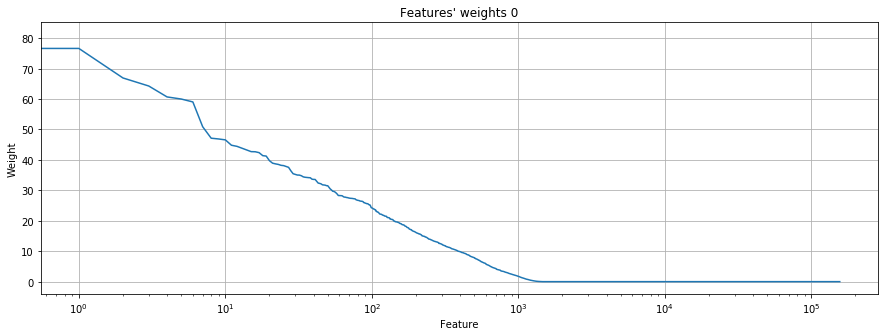
\includegraphics[width=\textwidth]{figures/conf_matrices/ita_rel_logreg/ita_rel_logreg_fs.png}
	\caption{Features' weights of Logistic Regression classifier for relevance detection before features selection}
	\label{fig:ita_rel_logreg_fs}
\end{figure}

After features selection the scores, obtained with the model with $C$=1000, become:

% LR fs
\begin{figure}[H]
	\centering
	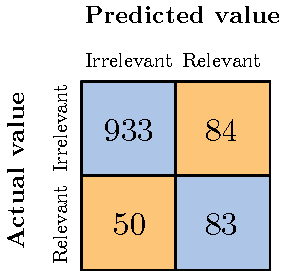
\includegraphics[scale=1]{figures/conf_matrices/ita_rel_logreg/ita_rel_logreg_afs.pdf}
	\label{fig:ita_rel_logreg_afs}
\end{figure}

% LR after fs
\begin{center}
	\begin{tabular}{ | c | c | } 
		\hline
		\textbf{F1-macro} & 0.553 \\
		\hline
		\textbf{Recall} & 0.624 \\ 
		\hline
		\textbf{Precision} & 0.497 \\ 
		\hline
	\end{tabular}
\end{center}

As in the previous situation, are shown the 25 most relevant features, obtained from the most heaviest weight of the Logistic Regression classifier. As before, the red weights are the ones concordant with the class "relevant". It is curious that most important features are different between SVM and Logistic Regression classifiers, and that there is no an effective interpretation of the features.

\begin{figure}[H]
	\centering
	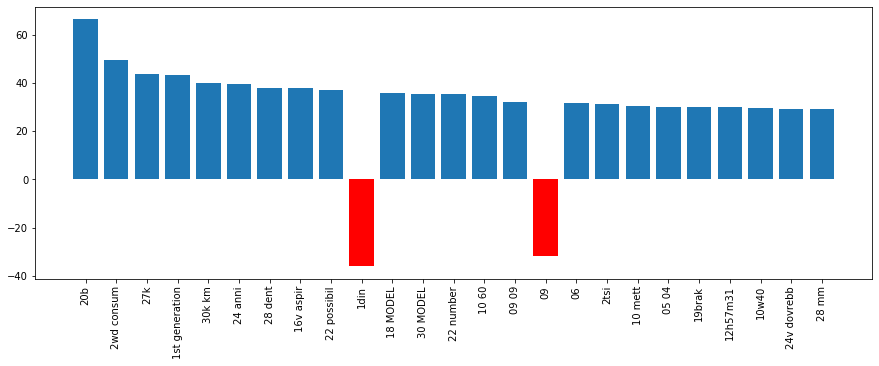
\includegraphics[width=\textwidth]{figures/conf_matrices/ita_rel_logreg/logreg_rel_best_feat.png}
	\caption{25 most relevant features of Logistic Regression relevance classifier after features selection}
	\label{fig:ita_rel_logreg_feat}
\end{figure}

From the confusion matrix it is possible to notice that the features selection improves mostly the precision, in fact it reduces the number of true positives from 91 to 84, while the recall remains similar.\\
Comparing the results with the SVM classifier, both reach similar results for what concerns the F1-macro score, but the Logistic Regression one gets a better recall, that makes it the preferable one.



\subsection{Sentiment Classification with SVM}

For sentiment classification it has been followed an approach similar to the one used for relevance detection: the same preprocessing and vectorization techniques have been applied, so the same is the dimension of the features space. The only thing that has been changed was the classifier, that became multiclass instead of binary. \\
A first result on validation data, obtained with the hyperparameter $C$=10, gave the following scores:

% SVM no fs
\begin{figure}[H]
	\centering
	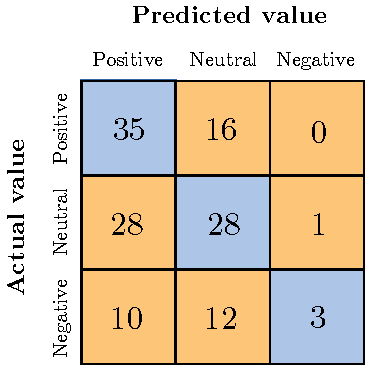
\includegraphics[scale=1]{figures/conf_matrices/ita_snt_svm/ita_snt_svm_bfs.pdf}
	\label{fig:ita_snt_svm_bfs}
\end{figure}

\begin{center}
	\begin{tabular}{ | c | c | } 
		\hline
		\textbf{F1-macro} & 0.422 \\
		\hline
		\textbf{F1-micro} & 0.496 \\ 
		\hline
	\end{tabular}
\end{center}

% fs
For simplicity in Figure \ref{fig:ita_snt_svm_fs} it has been shown just one of the three classifiers' weights that compose the one-versus-one multiclass classifier for sentiment classification. All graphics actually have the same shape, which is typical. Setting the cutoff values, respectively to 0.15, 0.1 and 0.1, the number of selected features become 9657, which is again much lower than initial dimension.

\begin{figure}[H]
	\centering
	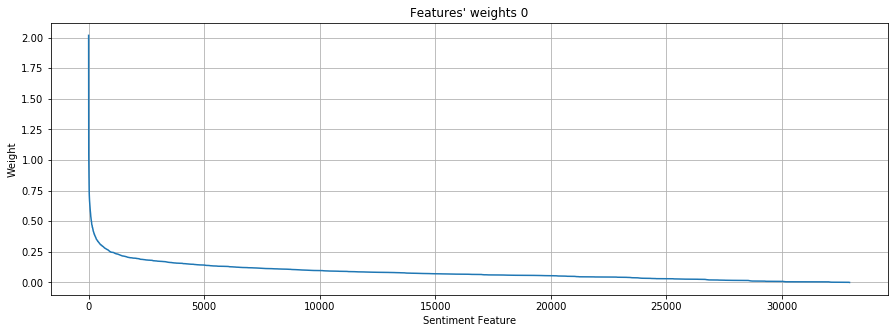
\includegraphics[width=\textwidth]{figures/conf_matrices/ita_snt_svm/ita_snt_svm_fs.png}
	\caption{Features' weights of SVM classifier for sentiment classification before features selection}
	\label{fig:ita_snt_svm_fs}
\end{figure}

% SVM fs
After features selection, the optimized model with $C$=10, the scores become:
\begin{figure}[H]
	\centering
	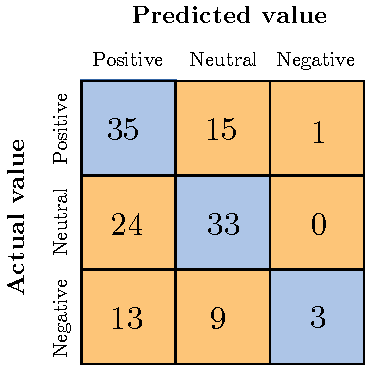
\includegraphics[scale=1]{figures/conf_matrices/ita_snt_svm/ita_snt_svm_afs.pdf}
	\label{fig:ita_snt_svm_afs}
\end{figure}

\begin{center}
	\begin{tabular}{ | c | c | } 
		\hline
		\textbf{F1-macro} & 0.451 \\
		\hline
		\textbf{F1-micro} & 0.534 \\ 
		\hline
	\end{tabular}
\end{center}

The scores notify a little improvement on the performance, that is easily seen in the classification of neutral class. Again, the scores are very different from the one seen for the Twitter's dataset, and the motivation have been already presented. Moreover, for this classification, the bias inducted for the negative class imbalance is visible on the confusion matrix: while positive and neutral classes perform quite well, for what concerns the negative class, the classifier tends to predict positive or neutral. This issue will be present in all other models, and it is characteristics the fact that the dataset is unbalanced.\\
This model has been used as baseline, in order to compare the effectiveness of the revised BPEF model, which results will be presented in the following paragraph.

\subsection{Sentiment Classification with Revised BPEF}

As mentioned, one goal was to improve the SVM classifier using the revised BPEF algorithm. The process was somehow the same as the one seen for Twitter sentiment classification. As previously discussed, features selection is based on information gain, and it has to be calculated before the classification, since it is not based on the classifiers' weights. Thus, for every feature parameter it has been calculated the information gain. All information trends actually have mostly the same graphics, so an example is shown in Figure \ref{fig:ita_bpef_fs_1}.

\begin{figure}[H]
	\centering
	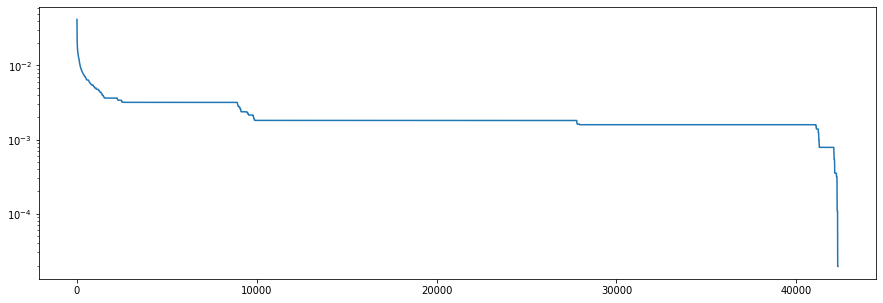
\includegraphics[width=\textwidth]{figures/conf_matrices/ita_snt_bpef/bpef_fs_1.png}
	\caption{Information Gain trend of the features.}
	\label{fig:ita_bpef_fs_1}
\end{figure}

% BPEF no fs
All BPEF models have been trained optimizing the following hyperparameters:
\begin{itemize}
	\item SVM: $C$ from $10^{-3}$ to $10^3$ with 7 exponentially evenly spaced values;
	\item Logistic Regression: $C$ from $10^{-3}$ to $10^3$ with 7 exponentially evenly spaced values;
	\item Random Forest: 
	\begin{itemize}
		\item Number of estimators: [201, 501]
		\item Maximum of looked features on split: [auto, $log_2$]
		\item Maximum depth of the tree: [10, 100]
		\item Split criterion: [gini, entropy]
	\end{itemize}
\end{itemize}

A first model training without features selection gives the following results:

\begin{figure}[H]
	\centering
	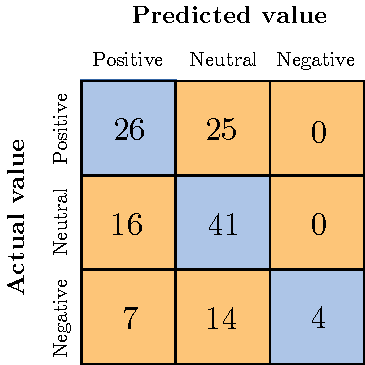
\includegraphics[scale=1]{figures/conf_matrices/ita_snt_bpef/ita_snt_bpef_bfs.pdf}
	\label{fig:ita_snt_bpef_bfs}
\end{figure}

\begin{center}
	\begin{tabular}{ | c | c | } 
		\hline
		\textbf{F1-macro} & 0.465 \\
		\hline
		\textbf{F1-micro} & 0.534 \\ 
		\hline
	\end{tabular}
\end{center}

% fs
It is possible to notice that even the model without features selection gives better results than the best SVM model, so this is actually an improvement.\\
Features selection has been made for each feature parameter selecting a cutoff value for information gain. The cutoff value, after some experiments was set to 0.0019, that is the value just above the flat area, and the number of selected features, which is different for each feature parameters is:

\begin{center}
	\begin{tabular}{ c  c  c } 
		\hline
		\textbf{Feature name} & \textbf{Word summarizing} & \textbf{\# Features} \\
		\hline
		word & false & 9.860 \\ 
		\hline
		word & true & 9.433 \\ 
		\hline
		pos & false & 11.580 \\ 
		\hline
		pos & true & 10.887 \\ 
		\hline
		swnt & false & 9.082 \\ 
		\hline
		swnt & true & 8.547 \\ 
		\hline
	\end{tabular}
\end{center}

After features selection the scores become:

% BPEF fs
\begin{figure}[H]
	\centering
	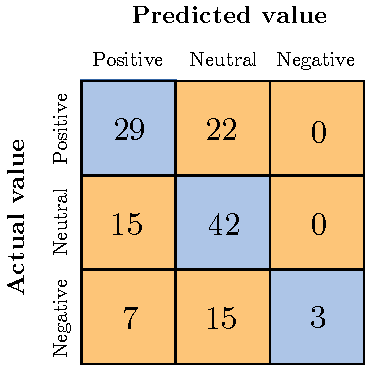
\includegraphics[scale=1]{figures/conf_matrices/ita_snt_bpef/ita_snt_bpef_afs.pdf}
	\label{fig:ita_snt_bpef_afs}
\end{figure}

\begin{center}
	\begin{tabular}{ | c | c | } 
		\hline
		\textbf{F1-macro} & 0.467 \\
		\hline
		\textbf{F1-micro} & 0.556 \\ 
		\hline
	\end{tabular}
\end{center}

With features selection it is possible to notice a little improvement of the performance, even if the bias inducted by the class unbalances is still present. However, the most important improvement is against the SVM sentiment classifier, in fact the overall F1-macro score improves by 0.016, improvement seen especially in the neutral classification. The final outcomes make this last model the preferred one for sentiment classification on the Italian automotive dataset.\\
For results evaluation, below are reported some mistakes on classification (between squared brackets the quotes):

\begin{itemize}
	\item \textbf{Positive predicted Neutral}: [\textit{@Matric: Ma l'hai ordinata come la volevi tu? Io mi sono dovuto accontentare di quello che c'era in arrivo (alla fine cambia solo il colore e motorizzazione e allestimento è quello voluto) ed è passato un mese e ancora nulla.}] \textit{Si come l'ho ordinata io con tutti gli accessori comunque il motore è molto silenzioso sembra a benzina}\\
	\item \textbf{Negative predicted Neutral}: [\textit{sicuro da giocarmi la mia GTA con il busso?la macchina nn me la giocherei nemmeno se mi dovessi indovinare la risp a questo quesito: chi è più BONA la Hunziker o tua nonna?}] \textit{ha fatto un passo indietro perchè va più veloce? la 159 temo che nemmeno con un motore sbarbato da un cofano maserati che a loro volta l'hanno dovuto rubare da dentro il centro ricerche ferrari riuscirà ad essere competitiva sul serio... qua dentro sembra un elefante la m3 figuriamoci una 159 gta... la prossima generazione di alfa magari sarà all'altezza del nome che porta ma per ora... } % TODO vedi se puoi tenere il commento
	\item \textbf{Negative predicted Neutral}: \textit{@Touareg 2.5 2.0 MultiJet II Aut. 4WD ( 170Cv ) : Trailhawk : 32.800€}
\end{itemize}

From these example come some difficulties and mistakes on manual labeling: In the second case, it is not explicit the reference of the engine of subject, in fact it is written that the car has poor performance, but the matter is not exactly the engine, so the correct label may be "neutral". In the third case, the comment is surely an error, since there is no sentiment polarity expressed by the user, so the correct label is "neutral". For both examples the classifier predicted the correct label (in the first it depends on the interpretation), even if the manual annotation was wrong, and it is a great result.



\subsection{4-labels Classification with SVM}

At this point, are available two classifier: the one responsible to relevance detection, and the one responsible to sentiment classification. Now the goal is to select the best model that best classifies all the four labels. The tested approaches involve the SVM classifier and the cascade classifier, built with the relevance detector and the sentiment classifier.\\
The first case follows the same approach seen for all SVM classifier, the only difference is that the output has four labels. The first result, obtained without features selection, with the optimal parameter $C$=1000, is the following:

% 4 labels SVM bfs
\begin{figure}[H]
	\centering
	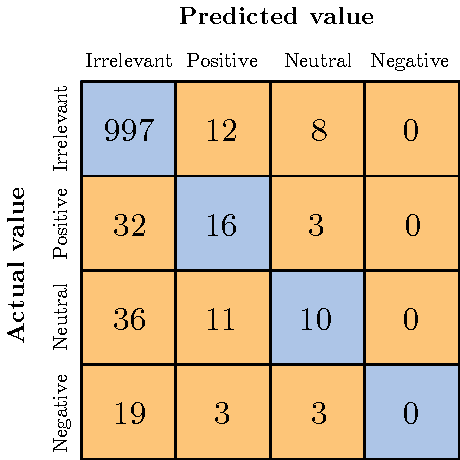
\includegraphics[scale=1]{figures/conf_matrices/ita_4l_svm/ita_4l_svm_bfs.pdf}
	\label{fig:ita_4l_svm_bfs}
\end{figure}

\begin{center}
	\begin{tabular}{ | c | c | } 
		\hline
		\textbf{F1-macro} & 0.385 \\
		\hline
		\textbf{F1-micro} & 0.890 \\ 
		\hline
	\end{tabular}
\end{center}

% fs
As usual, features selection consisted in the selection of the cutoff values, that have been chosen, for each of the six binary classifiers that compose the one-versus-one multiclass classifier, with respect to the features' weights that have the usual trend shown in Figure \ref{fig:svm4l_fs_1}.
\begin{figure}[H]
	\centering
	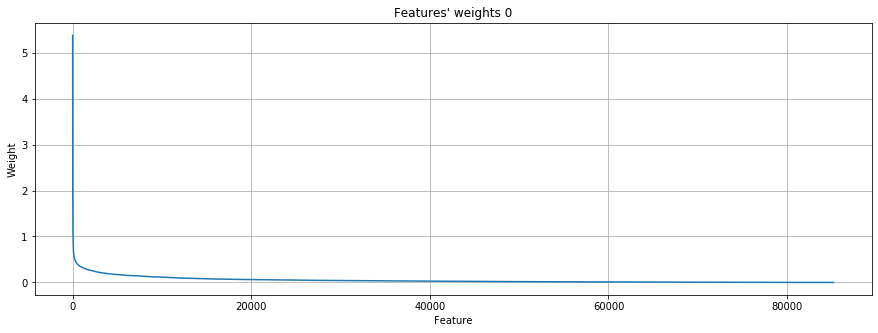
\includegraphics[width=\textwidth]{figures/conf_matrices/ita_4l_svm/svm4l_fs_1.png}
	\caption{Features' weight of the four labels SVM classifier.}
	\label{fig:svm4l_fs_1}
\end{figure}


% 4 labels SVM afs
After some tries for selecting the cutoff values, the total selected features become 45.088, which are a lot with respect to all the other features selection results. A new training with just the selected features gave the following results:

\begin{figure}[H]
	\centering
	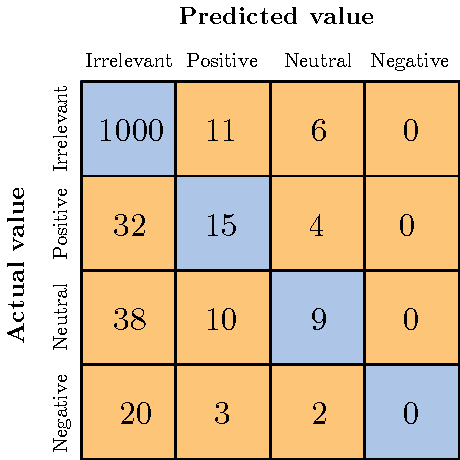
\includegraphics[scale=1]{figures/conf_matrices/ita_4l_svm/ita_4l_svm_afs.pdf}
	\label{fig:ita_4l_svm_afs}
\end{figure}

\begin{center}
	\begin{tabular}{ | c | c | } 
		\hline
		\textbf{F1-macro} & 0.378 \\
		\hline
		\textbf{F1-micro} & 0.890 \\ 
		\hline
	\end{tabular}
\end{center}

As it is possible to see, the performances seem quite poor, especially for the "negative" class, that is definitely ignored. The causes are surely related to the high imbalance across the classes, which is heavier than the past cases, in fact most errors are predicted as "irrelevant", that is a proof of the inducted bias. This confusion matrix is also a good example about why the micro score is not good to evaluate this particular problem, in fact the 89\% F1-micro score is misleading, because the actual performance are quite poor. \\
This result was taken as baseline in order to compare the results obtained with the cascade classifiers that will be presented in the following paragraphs.


\subsection{4-labels Classification with Cascade Classifier}

At this point, all blocks needed for build the cascade classifier are actually ready to be assembled. As previously said, the chosen classifier for relevance detection was the one that used Logistic Regression algorithm, because it was the one with better recall score, which means that it tends to detect better the topic treated on the comment. For comparison, on the second stage of the cascade classifier have been employed both SVM and the revised BPEF sentiment classifiers, trained after features selection.

\subsubsection{Cascade Classifier with SVM Sentiment Classifier}

Below are shown the scores on validation data obtained by the cascade classifier composed by the Logistic Regression relevance classification, and the SVM sentiment classifier.

% cascade SVM val
\begin{figure}[H]
	\centering
	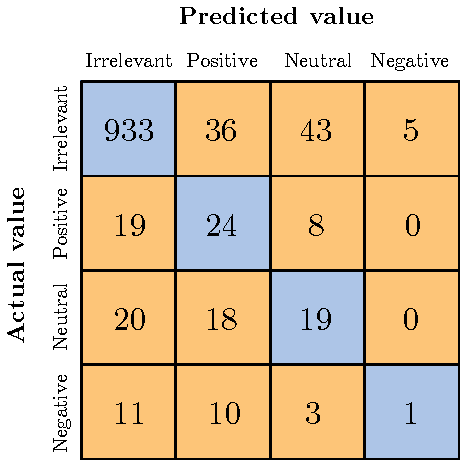
\includegraphics[scale=1]{figures/conf_matrices/ita_cascade_svm/ita_cascade_svm_val.pdf}
	\label{fig:ita_cascade_svm_val}
\end{figure}

\begin{center}
	\begin{tabular}{ | c | c | } 
		\hline
		\textbf{F1-macro} & 0.409 \\
		\hline
		\textbf{F1-micro} & 0.850 \\ 
		\hline
	\end{tabular}
\end{center}

The results show an improvements with respect to the baseline classifier, especially for what concerns the negative class, that is no more completely ignored. Even positive and neutral classes have shown some improvements, while the irrelevant class shows decreased performance. 




\subsubsection{Cascade Classifier with Revised BPEF Sentiment Classifier}

Below are shown the scores on validation data obtained by the cascade classifier composed by the Logistic Regression relevance classification, and the revised BPEF sentiment classifier.

% cascade BPEF val
\begin{figure}[H]
	\centering
	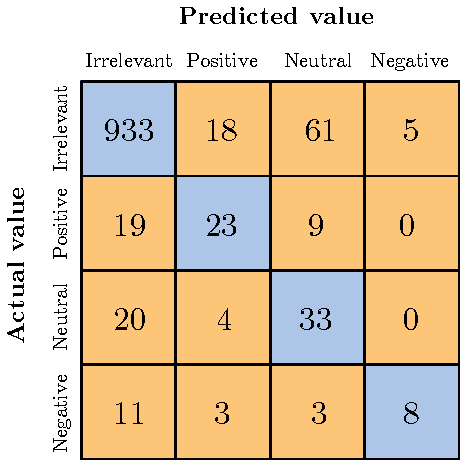
\includegraphics[scale=1]{figures/conf_matrices/ita_cascade_bpef/ita_cascade_bpef_val.pdf}
	\label{fig:ita_cascade_bpef_val}
\end{figure}

\begin{center}
	\begin{tabular}{ | c | c | } 
		\hline
		\textbf{F1-macro} & 0.556 \\
		\hline
		\textbf{F1-micro} & 0.867 \\ 
		\hline
	\end{tabular}
\end{center}

The scores present a huge improvements with respect to the both baseline classifier and the previous cascade classifier. The "negative" class now gives good results and may be considered reliable, while "positive" and "neutral" classes show better classification performance. It is also important to see that "big mistakes" don't happen, for instance just few negatives have been predicted positives and no positives has been predicted negatives. The presented scores lead to define this last classifier the preferable for topic relevance and sentiment classification, and it will be used for classify all the other categories.
% TODO comparative score con paper






\subsection{4-labels Classification with Test Data}

At this point, when the models have been chosen, it is a good practice to test them using new data, not yet involved in the model definition procedure. This data has been kept apart at the beginning, and consists in the actual test dataset. The following tests are used to verify that the models don't overfit validation data, and show how the model is going to work on real new comments.


\subsubsection{Cascade Classifier with SVM Sentiment Classifier}

The cascade classifier composed by the Logistic Regression relevance detector and SVM sentiment classifier gives the following results:

% cascade SVM test
\begin{figure}[H]
	\centering
	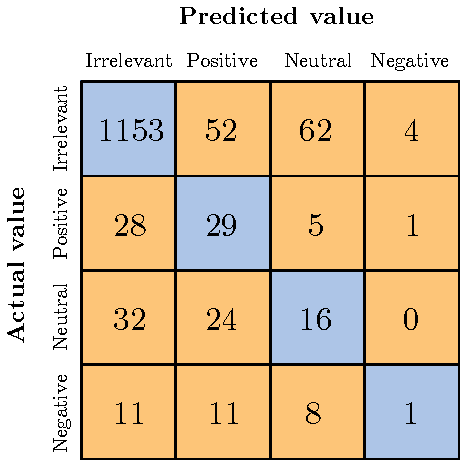
\includegraphics[scale=1]{figures/conf_matrices/ita_cascade_svm/ita_cascade_svm_tst.pdf}
	\label{fig:ita_cascade_svm_tst}
\end{figure}

\begin{center}
	\begin{tabular}{ | c | c | } 
		\hline
		\textbf{F1-macro} & 0.375 \\
		\hline
		\textbf{F1-micro} & 0.834 \\ 
		\hline
	\end{tabular}
\end{center}

The scores highlight a little decrease of the performance, but absolutely tolerable. It is possible to conclude that this model does not suffer from overfitting.


\subsubsection{Cascade Classifier with Revised BPEF Sentiment Classifier}

The same test has been made for the cascade classifier that involves the revised BPEF. It is important to get good scores because since it is the best model, a poor result will make the model unusable. The obtained scores are:

% cascade BPEF test
\begin{figure}[H]
	\centering
	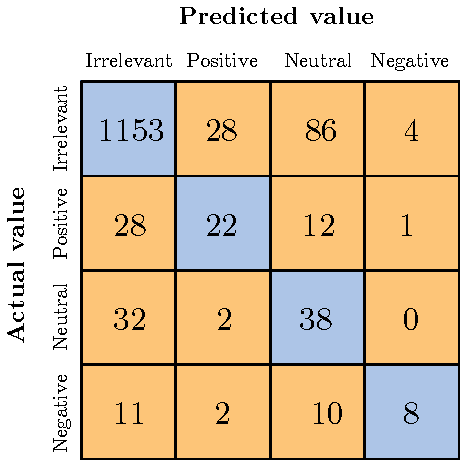
\includegraphics[scale=1]{figures/conf_matrices/ita_cascade_bpef/ita_cascade_bpef_tst.pdf}
	\label{fig:ita_cascade_bpef_tst}
\end{figure}

\begin{center}
	\begin{tabular}{ | c | c | } 
		\hline
		\textbf{F1-macro} & 0.503 \\
		\hline
		\textbf{F1-micro} & 0.850 \\ 
		\hline
	\end{tabular}
\end{center}

It is possible to conclude that, even if the scores are a little lower than the ones obtained with validation data, the model has still good values to be considered a good model for both relevance and sentiment classification.


\subsection{Classification with other Classes}

All the process seen for the classification of the class "engine" have been employed also for the training of the models for the classification of the classes "brand", "exteriors" and "support". Obviously it can be further extended for all the other topics. In this section, for sake of brevity, only main results will be presented along with some considerations. For every class, the subdivision of the comments between training, validation and test has been made maintaining the original distribution, subdividing the 80\% training and 20\% test, and the training was further divided into 80\% actual training and 20\% validation sets.

\subsubsection{Classification with "Brand" class}

The class "brand" was the one responsible to classify the sentiment about the manufacturers' perception. Its distribution about relevance is shown in Figure \ref{table:rel-dist-brand}.

\begin{table}[H]
	\centering
	\begin{tabular}{ | c  c  c | c | } 
		\hline
		& \textbf{Relevant} & \textbf{Irrelevant} & \textbf{Total} \\
		\hline
		\textbf{Training} & 880 & 3716 & 4.596 \\ 
		\hline
		\textbf{Validation} & 220 & 930 & 1.150 \\ 
		\hline
		\textbf{Test} & 274 & 1.163 & 1.437 \\
		\hline
	\end{tabular}
	\caption{Relevance distribution for class "brand".}
	\label{table:rel-dist-brand}
\end{table}

Again, imbalance is really heavy, so the same issues found for the "engine" class are expected. The distribution of the relevant comments is shown in Table \ref{table:snt-dist-brand}.

\begin{table}[H]
	\centering
	\begin{tabular}{ | c  c  c c | c | } 
		\hline
		& \textbf{Positives} & \textbf{Neutrals} & \textbf{Negatives} & \textbf{Total} \\
		\hline
		\textbf{Training} & 416 & 180 & 284 & 880 \\ 
		\hline
		\textbf{Validation} & 104 & 45 & 71 & 220 \\ 
		\hline
		\textbf{Test} & 130 & 56 & 88 & 274 \\
		\hline
	\end{tabular}
	\caption{Relevance distribution for class "brand".}
	\label{table:snt-dist-brand}
\end{table}

It is possible to see again imbalance in favor of the "positive" class, and lack of comments of the "neutral" class.\\
Starting from the final results, obtained on validation data with the cascade classifier, composed by the Logistic Regression relevance detector and the revised BPEF sentiment classifier, it is possible to notice lower performance than the one reached with the "engine" class, but still acceptable.


\begin{figure}[H]
	\centering
	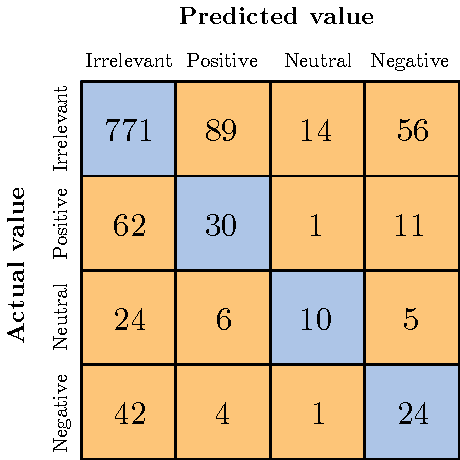
\includegraphics[scale=1]{figures/conf_matrices/ita_brand/ita_cascade_brand_bpef_val.pdf}
	\label{fig:ita_cascade_brand_bpef_val}
\end{figure}

\begin{center}
	\begin{tabular}{ | c | c | } 
		\hline
		\textbf{F1-macro} & 0.417 \\
		\hline
		\textbf{F1-micro} & 0.726 \\ 
		\hline
	\end{tabular}
\end{center}

The lower results comes mostly from the relevance detector, that was not very good to interpret comments belonging to the class "brand". In a way it is understandable, because sometimes comments that contain an opinion to a brand, express the subject implicitly, and this is a further difficulty for the classifier.\\
The performance of the Logistic Regression relevance classifier on validation data are:

\begin{figure}[H]
	\centering
	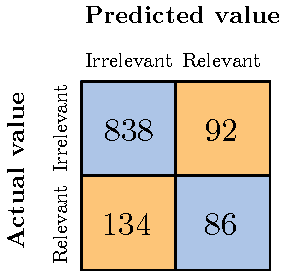
\includegraphics[scale=1]{figures/conf_matrices/ita_brand/ita_rel_brand_logreg_afs.pdf}
	\label{fig:ita_rel_brand_logreg_afs}
\end{figure}

\begin{center}
	\begin{tabular}{ | c | c | } 
		\hline
		\textbf{F1-macro} & 0.391 \\
		\hline
		\textbf{Recall} & 0.418 \\ 
		\hline
		\textbf{Precision} & 0.367 \\ 
		\hline
	\end{tabular}
\end{center}

As discussed, it presents performance lower than the one reached with the "engine" class. The second stage of the cascade classifier consisted in the revised BPEF, and it performance on the validation dataset are:

\begin{figure}[H]
	\centering
	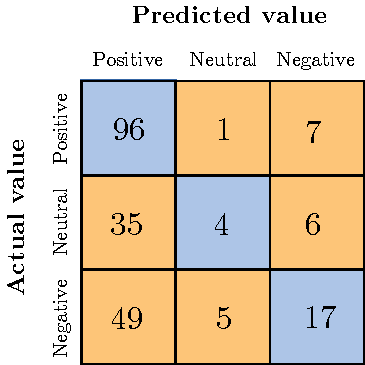
\includegraphics[scale=1]{figures/conf_matrices/ita_brand/ita_snt_brand_bpef_afs.pdf}
	\label{fig:ita_snt_brand_bpef_afs}
\end{figure}

\begin{center}
	\begin{tabular}{ | c | c | } 
		\hline
		\textbf{F1-macro} & 0.386 \\
		\hline
		\textbf{F1-micro} & 0.532 \\ 
		\hline
	\end{tabular}
\end{center}

From the confusion matrix it is possible to conclude that the classifier is affected by some bias, due to the imbalance to the positive class.\\
Finally, the classification with all four labels on test data gave the following results:

\begin{figure}[H]
	\centering
	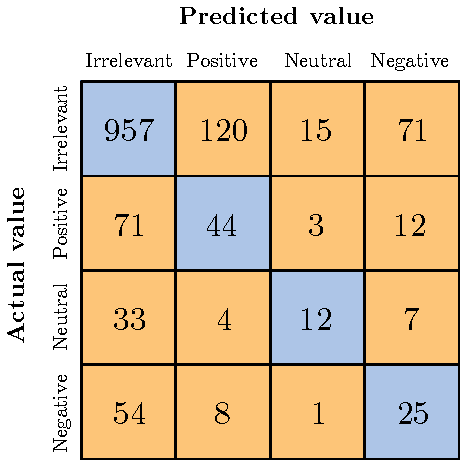
\includegraphics[scale=1]{figures/conf_matrices/ita_brand/ita_cascade_brand_bpef_tst.pdf}
	\label{fig:ita_cascade_brand_bpef_tst}
\end{figure}

\begin{center}
	\begin{tabular}{ | c | c | } 
		\hline
		\textbf{F1-macro} & 0.412 \\
		\hline
		\textbf{F1-micro} & 0.722 \\ 
		\hline
	\end{tabular}
\end{center}

% todo rivedere la frase prima di "irrelevant"
The performance are still affected by the relevance detector that doesn't reach the comments with brand reference. However, bias on "positive" sentiment seems reduced, and a simple exploitation may be that the comments that were going to be classified with the bias, were before classified "irrelevant".\\\\
In conclusion, even if lower than the engine classifier, the performance still may be considered reliable, also because performance on test and validation data were comparable, so no overfitting seems to be present.



\subsubsection{Classification with "Exteriors" class}

The class "exteriors" was the one responsible for the sentiment classification about vehicles' aesthetics and all comments with exteriors references. The distribution about comments' relevance is:

\begin{table}[H]
	\centering
	\begin{tabular}{ | c  c  c | c | } 
		\hline
		& \textbf{Relevant} & \textbf{Irrelevant} & \textbf{Total} \\
		\hline
		\textbf{Training} & 554 & 4.042 & 4.596 \\ 
		\hline
		\textbf{Validation} & 139 & 1.011 & 1.150 \\ 
		\hline
		\textbf{Test} & 173 & 1.264 & 1.437 \\
		\hline
	\end{tabular}
	\caption{Relevance distribution for class "exteriors".}
	\label{table:rel-dist-exteriors}
\end{table}

In general, even if the imbalance is still important, there are many comments that are relevant about this class. Continuing, the sentiment distribution of relevant comments is shown in Table \ref{table:snt-dist-exteriors}.

\begin{table}[H]
	\centering
	\begin{tabular}{ | c  c  c c | c | } 
		\hline
		& \textbf{Positives} & \textbf{Neutrals} & \textbf{Negatives} & \textbf{Total} \\
		\hline
		\textbf{Training} & 272 & 124 & 160 & 556 \\ 
		\hline
		\textbf{Validation} & 68 & 31 & 40 & 139 \\ 
		\hline
		\textbf{Test} & 85 & 39 & 50 & 174 \\
		\hline
	\end{tabular}
	\caption{Relevance distribution for class "exteriors".}
	\label{table:snt-dist-exteriors}
\end{table}

The distribution shows an imbalance on the "positive" class, but the metric that may gives more problems is supposed to be the actual number of comments, which are not plenty.\\
The best results comes from the cascade classifier with Logistic Regression relevance detector and BPEF sentiment classifier. The scores on validation data are:

\begin{figure}[H]
	\centering
	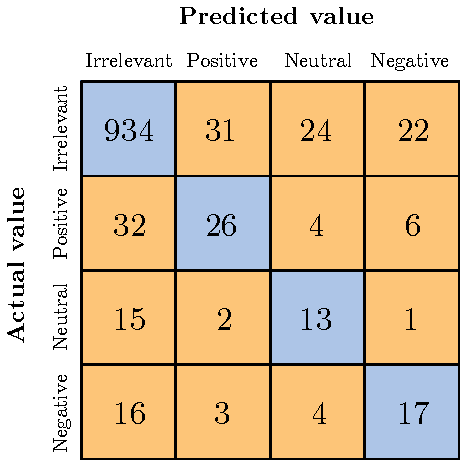
\includegraphics[scale=1]{figures/conf_matrices/ita_exteriors/ita_cascade_exteriors_bpef_val.pdf}
	\label{fig:ita_cascade_exteriors_bpef_val}
\end{figure}

\begin{center}
	\begin{tabular}{ | c | c | } 
		\hline
		\textbf{F1-macro} & 0.517 \\
		\hline
		\textbf{F1-micro} & 0.861 \\ 
		\hline
	\end{tabular}
\end{center}

The results show performance that are close to the one reached with the class "engine", and actually good. Some problems comes again from the relevance classification, which performance on validation data are:

\begin{figure}[H]
	\centering
	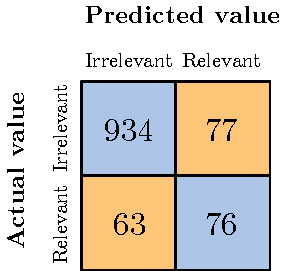
\includegraphics[scale=1]{figures/conf_matrices/ita_exteriors/ita_rel_exteriors_logreg_afs.pdf}
	\label{fig:ita_rel_exteriors_logreg_afs}
\end{figure}

\begin{center}
	\begin{tabular}{ | c | c | } 
		\hline
		\textbf{F1-macro} & 0.521 \\
		\hline
		\textbf{Recall} & 0.547 \\ 
		\hline
		\textbf{Precision} & 0.497 \\ 
		\hline
	\end{tabular}
\end{center}

The second stage with revised BPEF model gave the following results:

\begin{figure}[H]
	\centering
	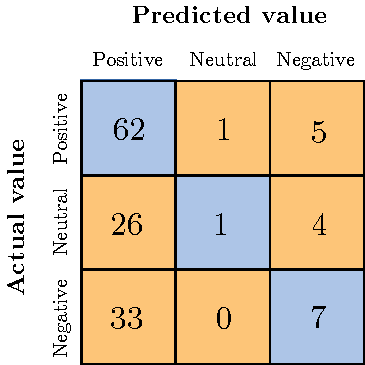
\includegraphics[scale=1]{figures/conf_matrices/ita_exteriors/ita_snt_exteriors_bpef_afs.pdf}
	\label{fig:ita_snt_exteriors_bpef_afs}
\end{figure}

\begin{center}
	\begin{tabular}{ | c | c | } 
		\hline
		\textbf{F1-macro} & 0.322 \\
		\hline
		\textbf{F1-micro} & 0.504 \\ 
		\hline
	\end{tabular}
\end{center}

The classifier actually suffers from the imbalance to the "positive" class, in fact most "negatives" and "neutrals" are classified as "positive". Even in this case the fact that poor results on classification are translated into good ones on the four label case can be explained in the fact that comments that were going to be classified wrongly, were before annotated as "irrelevant". These facts may be considered lucky cases, but another point of view may be that these comments are actually ambiguous or sufficiently "dirty" to be classifies "irrelevant".\\
Finally, classification on test data remarks the good final performance, that are:

\begin{figure}[H]
	\centering
	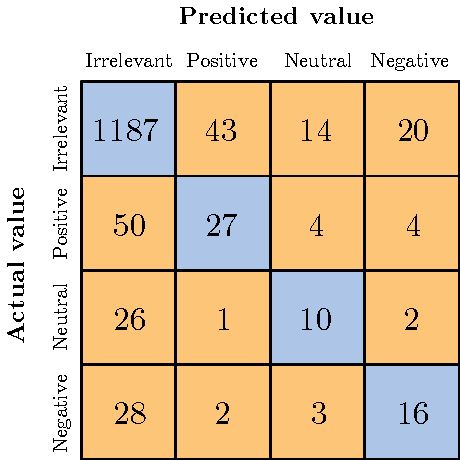
\includegraphics[scale=1]{figures/conf_matrices/ita_exteriors/ita_cascade_exteriors_bpef_tst.pdf}
	\label{fig:ita_cascade_exteriors_bpef_tst}
\end{figure}

\begin{center}
	\begin{tabular}{ | c | c | } 
		\hline
		\textbf{F1-macro} & 0.477 \\
		\hline
		\textbf{F1-micro} & 0.863 \\ 
		\hline
	\end{tabular}
\end{center}

The results are comparable to the ones reached with validation data, so the results can be considered out of overfitting and most importantly reliable.

\subsubsection{Classification with "Support" class}

The last class to be handled was the "support" one. It consists on the comments that regard reference about the customer care. The relevance class distribution is shown in Table \ref{table:rel-dist-support}. 

\begin{table}[H]
	\centering
	\begin{tabular}{ | c  c  c | c | } 
		\hline
		& \textbf{Relevant} & \textbf{Irrelevant} & \textbf{Total} \\
		\hline
		\textbf{Training} & 344 & 4.294 & 4.638 \\ 
		\hline
		\textbf{Validation} & 86 & 1.063 & 1.149 \\ 
		\hline
		\textbf{Test} & 108 & 1.288 & 1.396 \\
		\hline
	\end{tabular}
	\caption{Relevance distribution for class "support".}
	\label{table:rel-dist-support}
\end{table}

The sentiment distribution of relevant comments is shown in Table \ref{table:rel-dist-support}.

\begin{table}[H]
	\centering
	\begin{tabular}{ | c  c  c c | c | } 
		\hline
		& \textbf{Positives} & \textbf{Neutrals} & \textbf{Negatives} & \textbf{Total} \\
		\hline
		\textbf{Training} & 68 & 116 & 160 & 344 \\ 
		\hline
		\textbf{Validation} & 17 & 29 & 40 & 86 \\ 
		\hline
		\textbf{Test} & 22 & 36 & 50 & 108 \\
		\hline
	\end{tabular}
	\label{table:snt-dist-support}
	\caption{Sentiment distribution of relevant comments for class "support".}
\end{table}

For this class is visible an imbalance to the "negative" sentiment polarity, and again a lack of relevant comments.\\
the best performance were reached again with the cascade classifier with Logistic Regression relevance detector, and the revised BPEF sentiment classifier. The scores on validation data are:

\begin{figure}[H]
	\centering
	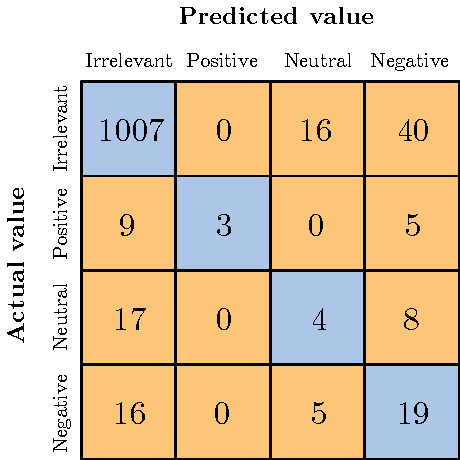
\includegraphics[scale=1]{figures/conf_matrices/ita_support/ita_cascade_support_bpef_val.pdf}
	\label{fig:ita_cascade_support_bpef_val}
\end{figure}

\begin{center}
	\begin{tabular}{ | c | c | } 
		\hline
		\textbf{F1-macro} & 0.435 \\
		\hline
		\textbf{F1-micro} & 0.899 \\ 
		\hline
	\end{tabular}
\end{center}

That are obtained with the Logistic Regression relevance detector that gave the following scores on validation data:

\begin{figure}[H]
	\centering
	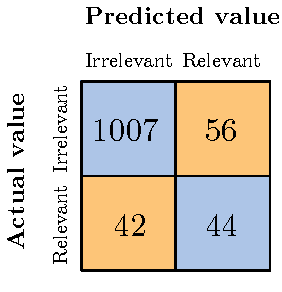
\includegraphics[scale=1]{figures/conf_matrices/ita_support/ita_rel_support_logreg_afs.pdf}
	\label{fig:ita_rel_support_logreg_afs}
\end{figure}

\begin{center}
	\begin{tabular}{ | c | c | } 
		\hline
		\textbf{F1-macro} & 0.473 \\
		\hline
		\textbf{Recall} & 0.512 \\ 
		\hline
		\textbf{Precision} & 0.440 \\ 
		\hline
	\end{tabular}
\end{center}

And the revised BPEF that gave the following scores on validation data:

\begin{figure}[H]
	\centering
	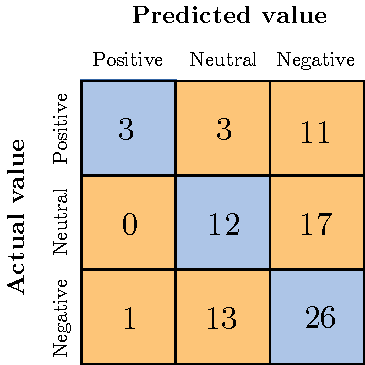
\includegraphics[scale=1]{figures/conf_matrices/ita_support/ita_snt_support_bpef_afs.pdf}
	\label{fig:ita_snt_support_bpef_afs}
\end{figure}

\begin{center}
	\begin{tabular}{ | c | c | } 
		\hline
		\textbf{F1-macro} & 0.420 \\
		\hline
		\textbf{F1-micro} & 0.477 \\ 
		\hline
	\end{tabular}
\end{center}

The mentioned imbalance on the "negative" polarity inducted a bias that has repercussions on the classification, in fact most errors fall on the negative side of the confusion matrix. The cascade classifier on new test data gave the following results:

\begin{figure}[H]
	\centering
	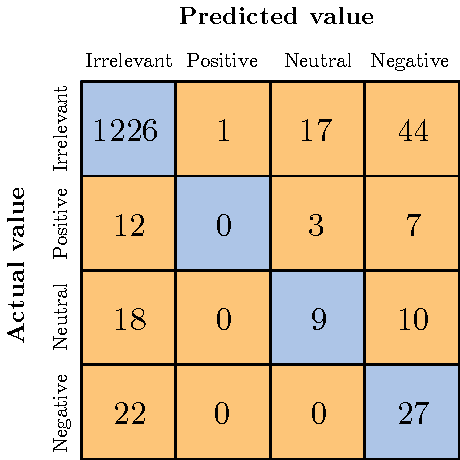
\includegraphics[scale=1]{figures/conf_matrices/ita_support/ita_cascade_support_bpef_tst.pdf}
	\label{fig:ita_cascade_support_bpef_tst}
\end{figure}

\begin{center}
	\begin{tabular}{ | c | c | } 
		\hline
		\textbf{F1-macro} & 0.406 \\
		\hline
		\textbf{F1-micro} & 0.907 \\ 
		\hline
	\end{tabular}
\end{center}

That again seem to be out of overfitting, having the scores similar to the one reached on validation data. Even for this case the model can be considered reliable.

